\documentclass[12pt,titlepage]{article}

\usepackage{geometry}

\usepackage[LGR, T1]{fontenc}
\usepackage[utf8]{inputenc}
\usepackage[greek,english]{babel}
\usepackage{alphabeta}

\usepackage{xcolor}
\definecolor{anti-flashwhite}{rgb}{0.95, 0.95, 0.96}
\usepackage{minted}
\usemintedstyle{friendly}
\setminted{bgcolor=anti-flashwhite,breaklines}

\usepackage{graphicx}
\graphicspath{{../plots/}}
\usepackage{caption}
\captionsetup{labelsep=space}

\begin{document}

\title{Συστήματα Παράλληλης Επεξεργασίας\\
    Άσκηση 3}
\author{Αλέξιος Ζαμάνης\\
    03115010\\
    Παναγιώτης Ζώγας\\
    03115191}
\date{\selectlanguage{greek}\today}

\maketitle

\section{Λογαριασμοί Τράπεζας}

Στο πρώτο μέρος της άσκησης έχουμε μια στοιχειώδη υλοποίηση τραπεζικών
λογαριασμών. Συγκεκριμένα, υπάρχει ένας πίνακας λογαριασμών και ένα σύνολο
νημάτων που εκτελούν λειτουργίες (προσθέσεις εν προκειμένω) στα στοιχεία του
πίνακα. Ο πίνακας έχει μήκος ίσο με το πλήθος των νημάτων και κάθε νήμα επιτελεί
λειτουργίες μόνο σε ένα λογαριασμό. Ως εκ τούτου, δεν υπάρχει μνήμη που
μοιράζεται μεταξύ των νημάτων (τουλάχιστον από προγραμματιστική άποψη), οπότε
δεν υπαρχει ανάγκη για συγχρονισμό.

Δεδομένης της απουσίας συγχρονισμού και της ανεξαρτησίας μεταξύ των νημάτων
περιμένουμε η αύξηση των νημάτων να οδηγεί σε ανάλογη αύξηση του throughput.
Αναμένουμε δηλαδή μια σχεδόν γραμμική σχέση μεταξύ πλήθους νημάτων και
throughput.

Εκτελούμε μετρήσεις του throughput για διαφορετικά πλήθη νημάτων και
διαφορετικές τοποθετήσεις των νημάτων αυτών στους διαθέσιμους πυρήνες. Τα
αποτελέσματα φαίνονται στο αριστερό τμήμα του σχήματος 1.

\begin{figure}[h!]
    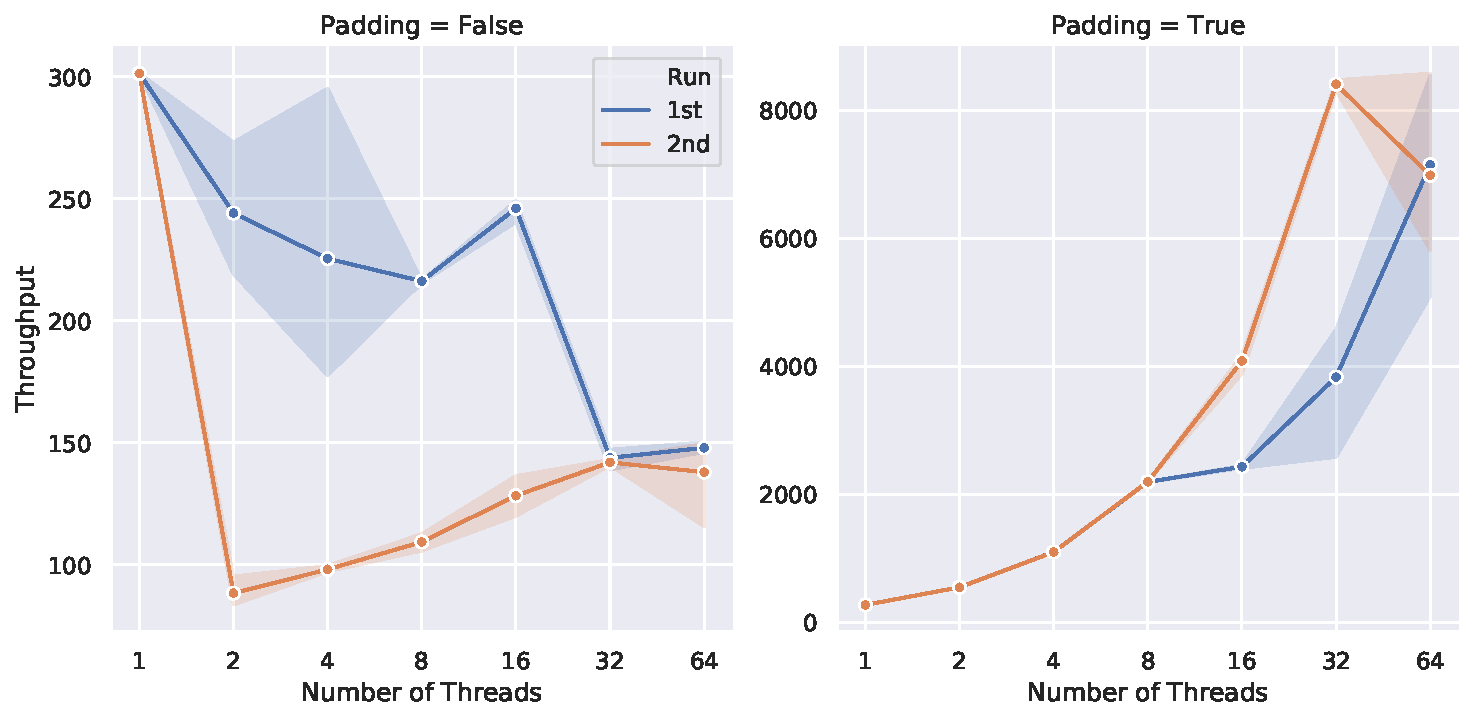
\includegraphics[width=\textwidth]{z1.pdf}
    \selectlanguage{greek}\caption{}
\end{figure}

Είναι σαφές ότι τα αποτελέσματα δεν είναι τα αναμενόμενα. Αρχικά παρατηρούμε ότι
η παράλληλη εκτέλεση, ανεξαρτήτως του πλήθους των νημάτων, χειροτερεύει την
επίδοση (αντί να την βλετιώνει).

Η εξήγηση έγκειται στην υλοποίηση του cache coherence στα μοντέρνα πολυπύρηνα
συστήματα. Δεδομένου ότι ένα block της cache είναι 64 bytes, ενώ ένας unsigned
int έχει μέγεθος μόλις 4 bytes, ένα block της cache θα περιέχει 16 στοιχεία του
πίνακα. Για να εξασφαλισθεί το coherence, κάθε μεταβολή ενός λογαριασμού από ένα
νήμα θα οδηγεί σε invalidation των αντιγράφων των (ανεξάρτητων) λογαριασμών στις
cache 15 άλλων νημάτων. Έχουμε δηλαδή false sharing. Σαν αποτέλεσμα θα υπάρχει
αυξημένη κίνηση στο bus, ενώ ουσιαστικά κάθε νήμα θα πρέπει σε (σχεδόν) κάθε
ανάγνωση να διαβάζει από κατώτερα τμήματα της ιεραρχίας μνήμης (αντί για την
cache του).

Αξίζει μάλιστα να παρατηρήσουμε τη διαφορά μεταξύ των 2 εκτελέσεων. Στην 1η
εκτέλεση τοποθετούμε τα νήματα όσο πιο κοντά γίνεται, ενώ στη 2η τα
απομακρύνουμε όσο περισσότερο μπορούμε. Με άλλα λόγια, στην 1η εκτέλεση
γεμίζουμε ένα socket (πρώτα 1 νήμα σε κάθε πυρήνα, έπειτα 2) πριν αρχίσουμε να
αναθέτουμε νήματα στο επόμενο. Αντίθετα, στη 2η εκτέλεση αναθέτουμε με
round-robin τρόπο νήματα στoυς πυρήνες κάθε socket (και μετά στα hardware
threads κάθε πυρήνα).

Σαν αποτέλεσμα από 2 μέχρι 16 νήματα η 1η εκτέλεση είναι σαφώς καλύτερη από τη
2η. Καθώς περιορίζουμε τα νήματα σε ένα μόνο socket, τα invalidations βρίσκονται
εντοπισμένα και πρέπει να διαδοθούν μέχρι την L3 cache. Αντίθετα, όταν τα νήματα
είναι διάσπαρτα σε όλα τα sockets, τα invalidations πρέπει να φτάσουν μέχρι την
κύρια μνήμη, αυξάνοντας τόσο την κίνηση στο bus, όσο και το χρόνο προσπέλασης
μιας θέσης μνήμης. Σημειώνουμε ότι στα 32 νήματα οι εκτελέσεις ταυτίζονται,
καθώς το false sharing επηρεάζει μόνο δεκαεξάδες διαδοχικών νημάτων. Έτσι, είτε
οι 2 δεκαεξάδες τοποθετηθούν σε 1 socket (όπως στην 1η εκτέλεση), είτε σε 2
(όπως στη 2η), δεν εμφανίζεται false sharing μεταξύ των sockets.

Για να αποφύγουμε το false sharing χρησιμοποιούμε padding, ώστε κάθε λογαριασμός
να καταλαμβάνει 64 (αντί για 4) bytes, ήτοι να έχει ένα δικό του block στην
cache. Στη C γράφουμε:

\begin{minted}{C}
struct {
    unsigned int value; /* 4 bytes */
    char padding[64 - sizeof(unsigned int)]; /* 60 bytes */
} accounts[MAX_THREADS];
\end{minted}

Επαναλαμβάνουμε τις μετρήσεις μας και λαμβάνουμε τα αποτελέσματα που φαίνονται
στο δεξί τμήμα του σχήματος 1.

Παρατηρούμε ότι πλέον πράγματι έχουμε επιτύχει την επιθυμητή κλιμάκωση του
throughput. Συγκεκριμένα παρατηρούμε μια σχεδόν γραμμική κλιμάκωση μέχρι τα 8
νήματα στην 1η εκτέλεση και μέχρι τα 32 νήματα στη 2η. Η διαφορά ανάμεσα στις 2
εκτελέσεις και η αποτυχία κλιμάκωσης της 1ης εκτέλεσης στα 64 νήματα οφείλονται
στο hyper-threading. Είναι σαφές ότι η εκτέλεση σε διαφορετικούς φυσικούς
πυρήνες (2η εκτέλεση) έχει σημαντικά καλύτερη επίδοση από την εκτέλεση σε
διαφορετικούς λογικούς πυρήνες (1η εκτέλεση). Μάλιστα φαίνεται πως η αύξηση από
32 νήματα σε ανεξάρτητους πυρήνες σε 64 νήματα στους ίδιους πυρήνες όχι μόνο δεν
βελτιώνει την επίδοση, αλλά ίσως και να τη χειροτερεύει.

\newpage

\section{Αμοιβαίος Αποκλεισμός - Κλειδώματα}

Στο δεύτερο μέρος της άσκησης έχουμε μια συνδεδεμένη λίστα, την οποία διαβάζουν
πολλά νήματα ταυτόχρονα. Δεδομένου ότι η λίστα δε μεταβάλλεται, δεν υπάρχει
ανάγκη για αμοιβαίο αποκλεισμό. Παραταύτα, ορίζουμε την αναζήτηση στη λίστα ως
κρίσιμο τμήμα και εφαρμόζουμε μια coarse-grained προσέγγιση. Ήτοι κάθε νήμα
κλειδώνει πριν ξεκινήσει την αναζήτηση και ξεκλειδώνει αφού την ολοκληρώσει.

Στόχος μας είναι να μελετήσουμε τους ίδιους τους μηχανισμούς κλειδώματος.
Συγκρίνουμε 5 διαφορετικούς μηχανισμούς, 3 εκ των οποίων υλοποιούμε εμείς. Στη
συνέχεια θα συζητήσουμε τις υλοποιήσεις και τα αποτελέσματα των μετρήσεών μας.

\subsection{Υλοποιήσεις}

\subsubsection{Pthread lock}

Η υλοποίηση του Pthread lock βασίζεται στο pthread\_spinlock\_t που προσφέρει η
ομώνυμη βιβλιοθήκη της C. Στην πραγματικότητα η υλοποίηση είναι τετριμμένη και
βασίζεται στην αντιστοίχηση των συναρτήσεων του δοθέντος interface στις
κατάλληλες συναρτήσεις τις βιβλιοθήκης. Έχουμε επομένως:

\begin{minted}{C}
struct lock_struct {
    pthread_spinlock_t state;
};

lock_t *lock_init(int nthreads) {
    lock_t *lock;

    XMALLOC(lock, 1);
    pthread_spin_init(&lock->state, PTHREAD_PROCESS_PRIVATE);
    return lock;
}

void lock_free(lock_t *lock) {
    pthread_spin_destroy(&lock->state);
    XFREE(lock);
}

void lock_acquire(lock_t *lock) {
    pthread_spin_lock(&lock->state);
}

void lock_release(lock_t *lock) {
    pthread_spin_unlock(&lock->state);
}
\end{minted}

\subsubsection{TTAS lock}

Το TTAS lock αποτελεί βελτιστοποίηση του TAS lock. Στην ουσία προσπαθούμε να
αποφύγουμε τις συνεχόμενες εγγραφές που προκαλεί η
\_\_sync\_lock\_test\_and\_set, καθώς το ίδιο το lock είναι μοιραζόμενος πόρος
μεταξύ όλων των νημάτων. Επομένως, λόγω του cache coherence κάθε εγγραφή κάνει
invalidate όλες τις υπόλοιπες cache και, εν τέλει, όλα τα νήματα καταλήγουν να
διαβάζουν συνεχώς από την κύρια μνήμη αντί για τις cache τους (ενώ αυξάνει
δραματικά και η κίνηση στο bus).

Για να το επιτύχουμε αυτό αντικαθιστούμε το spinning με ένα loop που μόνο
διαβάζει την κατάσταση του lock, μέχρι να το δει ξεκλείδωτο. Τότε δοκιμάζει να
το λάβει με την \_\_sync\_lock\_test\_and\_set. Αν επιτύχει επιστρέφει, ενώ αν
αποτύχει (πρόλαβε κάποιο άλλο νήμα) επαναλαμβάνει τη διαδικασία. Έχουμε δηλαδή:

\begin{minted}{C}
void lock_acquire(lock_t *lock) {
    lock_t *l = lock;

    for (;;) {
        while (l->state == LOCKED)
            /* do nothing */;
        if (__sync_lock_test_and_set(&l->state, LOCKED) == UNLOCKED)
            return;
    }
}
\end{minted}

Αξίζει να σημειωθεί ότι, ενώ έχουμε μειώσει πολύ τα invalidations σε σχέση με
το απλό TAS lock, η ελευθέρωση του lock με \_\_sync\_lock\_release και οι
επακόλουθες εκτελέσεις \_\_sync\_lock\_test\_and\_set από τα νήματα θα οδηγήσουν
σε μια (σύντομη ευτυχώς) μεταβατική περίοδο με δραματικά πολλά invalidations.

\subsubsection{Array lock}

Το array lock μοιάζει αρκετά, τόσο στην υλοποίηση όσο και στην φιλοσοφία, στο
δοθέν CLH lock. Η ιδέα πίσω από τα 2 αυτά locks, που ανήκουν στην ευρύτερη
κατηγορία των queue locks, είναι η χρήση μιας ουράς αναμονής, στην οποία
περιμένουν τα νήματα για να μπουν στο κρίσιμο τμήμα. Σαν αποτέλεσμα κάθε νήμα
ζητά (άμεσα) το κλείδωμα μόνο από τον προηγούμενό του στην ουρά, σε αντίθεση με
τα locks που είδαμε μέχρι τώρα, στα οποία όλα τα νήματα πάλευαν για ένα και
μοναδικό κλείδωμα (στην ουσία μία θέση μνήμης). Αυτή η point-to-point
προσέγγιση προσπαθεί να ελαχιστοποιήσει την ανάγκη για invalidations λόγω του
cache coherence, περιορίζοντάς την μόνο στις cache 2 νημάτων τη φορά.

Ορίζουμε στην ουσία έναν (κυκλικό) πίνακα με μήκος ίσο με το πλήθος των νημάτων
που ζητούν πρόσβαση στο κρίσιμο τμήμα. Επίσης έχουμε μια μοιραζόμενη μεταβλητή
στην οποία κρατάμε την πρώτη άδεια θέση του πίνακα. Κάθε νήμα που θέλει να λάβει
το lock, διαβάζει και αυξάνει ατομικά αυτή τη μεταβλητή με την
\_\_sync\_fetch\_and\_add και αποθηκεύει τη θέση του σε μια τοπική (\_\_thread)
μεταβλητή του. Στη συνέχεια περιμένει με busy-wait να λάβει σήμα από τον
προηγούμενό του. Κατ' αντιστοιχία, κάθε νήμα που θέλει να αφήσει το lock
φεύγει από τη θέση που έχει καταλάβει και στέλνει σήμα στον επόμενό του.

Αξίζει να παρατηρηθεί η χρήση padding στις θέσεις του πίνακα, ώστε να αποφευχθεί
το false sharing. Εν τέλει σε C έχουμε:

\begin{minted}{C}
#define FALSE 0
#define TRUE 1

typedef struct {
    char locked; /* FALSE or TRUE. */
    char padding[63];
} array_node_t;

struct lock_struct {
    int tail;
    array_node_t *flag;
    int size;
};

__thread int mySlotIndex;

lock_t *lock_init(int nthreads) {
    lock_t *lock;
    array_node_t *flag;

    XMALLOC(lock, 1);
    XMALLOC(flag, nthreads);

    lock->size = nthreads;
    lock->tail = 0;
    lock->flag = flag;
    lock->flag[0].locked = TRUE;

    return lock;
}

void lock_free(lock_t *lock) {
    lock_t *l = lock;
    XFREE(l);
}

void lock_acquire(lock_t *lock) {
    lock_t *l = lock;

    mySlotIndex = __sync_fetch_and_add(&l->tail, 1) % l->size;

    while (l->flag[mySlotIndex].locked == FALSE)
        /* do nothing */;
}

void lock_release(lock_t *lock) {
    lock_t *l = lock;

    l->flag[mySlotIndex].locked = FALSE;
    l->flag[(mySlotIndex + 1) % l->size].locked = TRUE;
}
\end{minted}

\subsection{Μετρήσεις}

Εκτελούμε μετρήσεις του throughput για κάθε υλοποίηση μεταβάλλοντας το πλήθος
των νημάτων και το μέγεθος της λίστας και λαμβάνουμε τα αποτελέσματα που
φαίνονται στο σχήμα 2.

\begin{figure}[h!]
    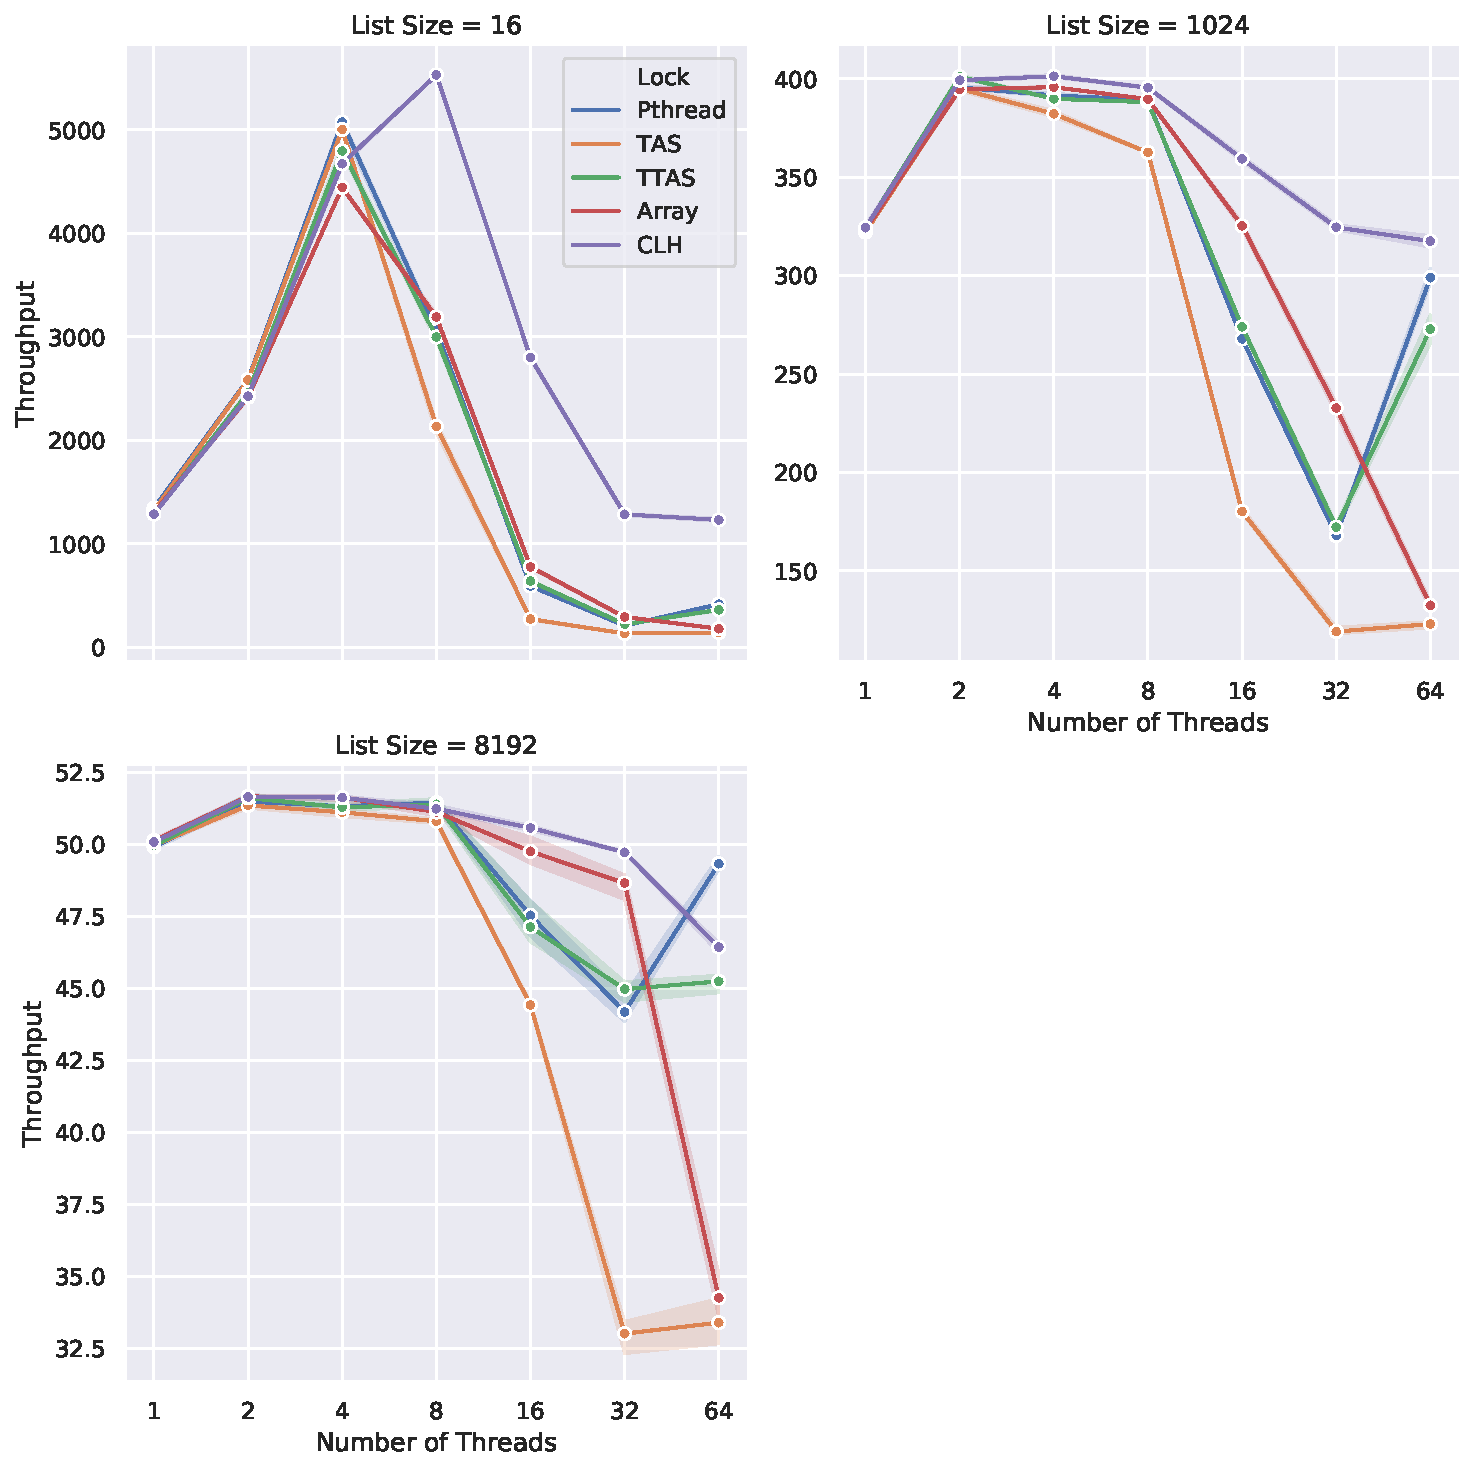
\includegraphics[width=\textwidth]{z2.pdf}
    \selectlanguage{greek}\caption{}
\end{figure}

Αρχικά είναι σαφές ότι καμία υλοποίηση δεν κλιμακώνει σε πάνω από 2 (ή 4 για τη
μικρή λίστα) νήματα (μόνο το CLH lock φαίνεται να κλιμακώνει μέχρι τα 8 νήματα
στη μικρή λίστα). Αντίθετα, η προσθήκη νημάτων μετά από κάποιο σημείο φαίνεται
να μειώνει δραματικά το συνολικό throughput. Μάλιστα είναι τόσο μεγάλη η διαφορά
σε σχέση με την υλοποίηση χωρίς locks που, παρότι τη μετρήσαμε, αδυνατούμε να
την παραστήσουμε στην ίδια κλίμακα. Τα παραπάνω βεβαίως πρέπει να εκληφθούν ως
αποτυχία του coarse-grained συγχρονισμού παρουσία πολλών νημάτων που ζητούν
μονίμως πρόσβαση στο ίδιο κρίσιμο τμήμα, παρά ως αποτυχία των ίδιων των
κλειδωμάτων. Ως εκ τούτου, θα μελετήσουμε τις διάφορες υλοποιήσεις συγκρίνοντας
τα σχετικά τους throughputs (και όχι ως απόλυτες τιμές).

Σε γενικές γραμμές βλέπουμε ότι μέχρι τα 8 νήματα οι διάφορες υλοποιήσεις
εμφανίζουν σχεδόν την ίδια επίδοση (εξαίρεση το TAS lock στη μεσαία λίστα, που
είναι σαφώς χειρότερο από τα υπόλοιπα). Για περισσότερα νήματα αρχίζουν να
ξεχωρίζουν το CLH ως το καλύτερο και το TAS ως το χειρότερο. Το Pthread lock
είναι πρακτικά ίδιο στη συμπεριφορά με το TTAS lock. Εξαιρεση αποτελούν τα 64
νήματα, όπου το Pthread lock φαίνεται να αποδίδει καλύτερα για μεγαλύτερες
λίστες, ξεπερνώντας μάλιστα ακόμα και το CLH lock στην μεγάλη λίστα (προφανώς η
υλοποίηση του εκμεταλλεύεται καλύτερα στο hyper-threading). Τέλος το array lock
είναι σε γενικές γραμμές το δεύτερο καλύτερο, με εξαίρεση τα 64 νήματα, όπου
καταλήγει το χειρότερο (στην πραγματικότητα εξίσου κακό με το TAS).

Τα αποτελέσματα αυτά είναι κάπως αναμενόμενα και αντιστοιχούν στη ολοένα και
καλύτερη διαχείριση του cache coherence από πλευράς των υλοποιήσεων μας.
Ξεκινήσαμε από το TAS lock που συνεχώς γράφει μια κοινή θέση μνήμης. Μετά
προχωρήσαμε στο TTAS lock που περιορίζει τις εγγραφές στη στιγμή της
απελευθέρωσης του lock και διεκδίκισής του από τα εν αναμονεί νήματα και τις
αντικαθιστά από συνεχείς αναγνώσεις. Τέλος καταλήξαμε στα 2 queue locks που
ελαχιστοποιούν τις εγγραφές, αντικαθιστώντας τη μοναδική θέση μνήμης από μια
ουρά αναμονής, στην οποία η διεκδίκηση γίνεται μόνο από ένα νήμα στο προηγούμενό
του (ήτοι πολλές αναγνώσεις και μία εγγραφή). Βέβαια δεν παύει να υπάρχει σημείο
(το τέλος της ουράς) που διεκδικείται από όλα τα νήματα (και επομένως πρέπει να
αποκτηθεί ατομικά), όμως αυτό αποκτάται άμεσα (δε συμβαίνει σε αυτό το
spinning).

Μεταξύ των queue locks το CLH lock είναι εμφανώς καλύτερο. Εικάζουμε πως η
διάκριση έγκειται στη χρήση μοιραζόμενης μνήμης στο array lock για την
αποθήκευση ολόκληρου του array, έναντι της χρήσης ιδιωτικών μεταβλητών από κάθε
νήμα στο CLH lock για την αποθήκευση μόλις 2 κόμβων της ουράς. Επιπλέον στο CLH
lock κάθε νήμα επαναχρησιμοποιεί πάντα έναν από τους 2 κόμβους που κατέχει, ενώ
στο array lock κάθε φορά καταλήγει σε μια τυχαία θέση στο array. Εκτιμούμε εν
τέλει πως η βελτιστότητα του CLH lock έγκειται σε καλύτερη αξιοποίηση της cache.

\newpage

\section{Τακτικές συγχρονισμού για δομές δεδομένων}

Στο τρίτο και τελευταίο μέρος της άσκησης χρησιμοποιούμε πάλι μια συνδεδμένη
λίστα. Τώρα ωστόσο κατασταλάζουμε στα Pthread locks και δοκιμάζουμε διάφορες
τεχνικές συχρονισμού που υπόσχονται καλύτερη επίδοση παρουσία νημάτων που
εκτελούν τόσο αναζητήσεις όσο και εγγραφές (προσθήκες ή διαγραφές) στοιχείων.
Στην ουσία προσπαθούμε σταδιακά να μειώνουμε τη χρήση των ίδιων των κλειδωμάτων.
Καταλήγουμε μάλιστα σε μια υλοποίηση που εξαλείφει τελείως τα κλειδώματα και
χρησιμοποιεί ατομικές εντολές αντί αυτών.

\subsection{Υλοποιήσεις}

\subsubsection{Fine-grained synchronization}

Η fine-grained υλοποίηση αποτελεί την πρώτη βελτίωση του coarse-grained
συγχρονισμού. Αντί να κλειδώνουμε όλη τη δομή, κλειδώνουμε μόνο τον κόμβο στον
οποίο βρισκόμαστε και τον προηγούμενό του. Απαιτείται πάντα να κλειδώνουμε 2
διαδοχικούς κόμβους, ώστε να μη συμβεί κάποια αλλαγή στον προηγούμενο κόμβο,
ενώ εμείς ξεκλειδώνουμε και ετοιμαζόμαστε να κλειδώσουμε τον επόμενο. Υπάρχει
δηλαδή η απαίτηση για hand-over-hand locking.

Προφανώς το lock δε βρίσκεται πλέον στη λίστα, αλλά κάθε κόμβος έχει το δικό του
lock, το οποίο αρχικοποιείται όταν δεσμεύεται ο κόμβος και καταστρέφεται όταν
ο κόμβος ελευθερώνεται. Ενδιαφέρον έχει η remove, στην οποία υλοποιείται η
τεχνική κλειδώματος. Αρχικά κλειδώνουμε την κεφαλή. Στη συνέχεια κλειδώνουμε το
πρώτο στοιχείο. Συνεχίζουμε την αναζήτηση βάσει του κλειδιού μας, ξεκλειδώνοντας
κάθε φορά τον προηγούμενο κόμβο και κλειδώνοντας τον επόμενο (στο μεταξύ ο ίδιος
ο κόμβος παραμένει κλειδωμένος). Μόνο αφού έχουμε βρει και επεξεργαστεί το
στοιχείο που μας ενδιαφέρει απελευθερώνουμε τα κλειδιά (και τα 2 μαζί).

Αναφορικά με τα κλειδώματα, οι contains και add είναι πανομοιότυπες με την
remove, οπότε δεν τις παραθέτουμε. Έχουμε επομένως:

\begin{minted}{C}
typedef struct ll_node {
    int key;
    struct ll_node *next;
    pthread_spinlock_t lock;
} ll_node_t;

struct linked_list {
    ll_node_t *head;
};

static ll_node_t *ll_node_new(int key) {
    ll_node_t *ret;

    XMALLOC(ret, 1);
    ret->key = key;
    ret->next = NULL;
    pthread_spin_init(&ret->lock, PTHREAD_PROCESS_PRIVATE);

    return ret;
}

static void ll_node_free(ll_node_t *ll_node) {
    pthread_spin_destroy(&ll_node->lock);
    XFREE(ll_node);
}

int ll_remove(ll_t *ll, int key) {
    int ret = 0;
    ll_node_t *curr, *next;

    pthread_spin_lock(&ll->head->lock);
    curr = ll->head;
    next = curr->next;
    pthread_spin_lock(&next->lock);

    while (next->key < key) {
        pthread_spin_unlock(&curr->lock);
        curr = next;
        next = curr->next;
        pthread_spin_lock(&next->lock);
    }

    if (key == next->key) {
        ret = 1;
        curr->next = next->next;
        ll_node_free(next);
    }
    pthread_spin_unlock(&next->lock);
    pthread_spin_unlock(&curr->lock);

    return ret;
}
\end{minted}

\subsubsection{Optimistic synchronization}

Δυστυχώς το hand-over-hand locking εισάγει ένα σημαντικό overhead. Για να το
γλιτώσουμε εφαρμόζουμε την εξής τακτική: κλειδώνουμε μόνο όταν έχουμε βρει το
στοιχείο που μας ενδιαφέρει (όπως πριν, κλειδώνουμε το ίδιο το στοιχείο και το
προηγούμενό του) και, ενώ κατέχουμε τα locks, διασχίζουμε από την αρχή τη λίστα
και ελέγχουμε ότι δεν υπήρξε κάποια αλλαγή μέχρι να πάρουμε τα κλειδώματα. Ήτοι,
ότι ο επόμενος του προηγούμενου στοιχείου είναι το ίδιο το στοιχείο. Αν
αποτύχουμε, επαναλαμβάνουμε τη διαδικασία από την αρχή. Προφανώς, η τεχνική αυτή
έχει αξία μόνο αν η αισιοδοξία μας ότι θα επιτύχουμε είναι βάσιμη (λ.χ. δεν
προσπαθούν ταυτόχρονα πολλά νήματα να μεταβάλουν το ίδιο στοιχείο).

Πάλι από άποψη κλειδωμάτων οι contains, add και remove ταυτίζονται, οπότε
παραθέτουμε μόνο τη remove. Επιπλέον οι λοιπές δομές και συναρτήσεις παραμένουν
ως είχαν. Έχουμε λοιπόν:

\begin{minted}{C}
int validate(ll_t *ll, ll_node_t *curr, ll_node_t *next) {
    ll_node_t *node = ll->head;

    while (node->key <= curr->key) {
        if (node == curr)
            return next == curr->next;
        node = node->next;
    }

    return 0;
}

int ll_remove(ll_t *ll, int key) {
    int ret = 0;
    ll_node_t *curr, *next;
    int validated;

    for (;;) {
        curr = ll->head;
        next = curr->next;

        while (next->key < key) {
            curr = next;
            next = curr->next;
        }

        pthread_spin_lock(&curr->lock);
        pthread_spin_lock(&next->lock);
        if ((validated = validate(ll, curr, next)))
            if (key == next->key) {
                ret = 1;
                curr->next = next->next;
            }
        pthread_spin_unlock(&curr->lock);
        pthread_spin_unlock(&next->lock);

        if (validated)
            return ret;
    }
}
\end{minted}

\subsubsection{Lazy synchronization}

Παρά τη βελτίωση που επιφέρει ο αισιόδοξος συγχρονισμός, είναι εμφανές ότι το
validation επιφέρει σημαντική καθυστέρηση, δεδομένου ότι ξαναδιασχίζει τη λίστα.
Η οκνηρή προσέγγιση επιλύει αυτό το πρόβλημα ως εξής: κάθε νήμα που θέλει να
σβήσει ένα κόμβο (ακριβώς όπως στον αισιόδοξο συγχρονισμό) πρώτα τον σημειώνει
ως σβησμένο και μετά τον αφαιρεί από τη λίστα (εν δυνάμει θα μπορούσε οι
αφαιρέσεις να συμβαίνουν μαζικά κάποια άλλη στιγμή). Προφανώς απαιτείται ένα
flag σε κάθε κόμβο, το οποίο θα αρχικοποιείται σε false κατά τη δημιουργία του
κόμβου.

Σβήνοντας πρώτα λογικά και μετά φυσικά τους κόμβους, μπορούμε πλέον να
περιορίσουμε τα validations στη γειτονιά του προς επεξεργασία κόμβου.
Συγκεκριμένα ελέγχουμε αν ο ίδιος ο κόμβος ή ο προηγούμενός του έχουν σημειωθεί
ως σβησμένοι και αν ο επόμενος του προηγούμενου είναι ο ίδιος ο κόμβος.
Επιπλέον, με τη χρήση flags καταφέρνουμε να απαλλάξουμε την contains από τα
κλειδώματα. Αρκεί να διασχίζει τη λίστα όπως η σειριακή, με την επιπλέον
απαίτηση ότι ο ζητούμενος κόμβος, αν υπάρχει, δεν είναι σημειωμένος.

Όλες οι υπόλοιπες δομές και συναρτήσεις (μια εξ αυτών και η add) παραμένουν
αμετάβλητες και δεν παρατίθενται. Έχουμε:

\begin{minted}{C}
typedef struct ll_node {
    int key;
    struct ll_node *next;
    pthread_spinlock_t lock;
    int marked;
} ll_node_t;

static ll_node_t *ll_node_new(int key) {
    ll_node_t *ret;

    XMALLOC(ret, 1);
    ret->key = key;
    ret->next = NULL;
    pthread_spin_init(&ret->lock, PTHREAD_PROCESS_PRIVATE);
    ret->marked = 0;

    return ret;
}

int validate(ll_node_t *curr, ll_node_t *next) {
    return !curr->marked && !next->marked && next == curr->next;
}

int ll_contains(ll_t *ll, int key) {
    ll_node_t *curr = ll->head;
    int ret = 0;

    while (curr->key < key)
        curr = curr->next;

    ret = (key == curr->key && !curr->marked);
    return ret;
}

int ll_remove(ll_t *ll, int key) {
    int ret = 0;
    ll_node_t *curr, *next;
    int validated;

    for (;;) {
        curr = ll->head;
        next = curr->next;

        while (next->key < key) {
            curr = next;
            next = curr->next;
        }

        pthread_spin_lock(&curr->lock);
        pthread_spin_lock(&next->lock);
        if ((validated = validate(curr, next))) {
            if (key == next->key) {
                ret = 1;
                next->marked = 1;
                curr->next = next->next;
            }
        }
        pthread_spin_unlock(&next->lock);
        pthread_spin_unlock(&curr->lock);

        if (validated)
            return ret;
    }
}
\end{minted}

\subsubsection{Non-blocking synchronization}

Τελικό βήμα στην προσπάθειά μας να μειώσουμε τη χρήση των locks είναι η εξάλειψή
τους και η αντικατάστασή τους από ατομικές εντολές. Θα προσπαθήσουμε να
επεκτείνουμε προς αυτή την κατεύθυνση την οκνηρή υλοποίηση. Δεδομένου ότι
θέλουμε να ελέγχουμε και να τροποποιούμε ατομικά το δείκτη προς το επόμενο
στοιχείο και το flag, πρέπει να τα βλέπουμε ως μια μοναδική θέση μνήμης.

Επιλέγουμε να χρησιμοποιήσουμε ένα union με το δείκτη και το flag. Το δεύτερο το
ορίζουμε τύπου uintptr\_t, ώστε να μπορούμε να εφαρμόζουμε σε αυτό bitwise
operations. Στην ουσία χρησιμοποιούμε το λιγότερο σημαντικό (και αχρησιμοποίητο)
bit του δείκτη για να αποθηκεύουμε το flag. Για να λάβουμε ένα εκ των δύο πεδίων
εφαρμόζουμε μάσκα (bitwise and με \textasciitilde1 για το δείκτη και με 1 για το
flag). Ενθυλακώνουμε αυτές τις λειτουργίες σε getters για προγραμματιστική
ευκολία.

Ιδιαίτερο ενδιαφέρον εμφανίζουν οι add και remove. Σε αμφότερες η τροποποίηση
της δομής γίνεται χρήσει της compare\_and\_swap (που με τη σειρά της αποτελεί
έναν wrapper για την \_\_sync\_bool\_compare\_and\_swap που κρύβει τα bitwise
operations). Έτσι στην add βάζουμε τον προηγούμενο κόμβο να δείχνει στο νέο
κόμβο, μόνο αν δεν ήταν σημειωμένος ως σβησμένος και έδειχνε στον δικό μας
κόμβο. Αλλιώς αποτυγχάνουμε και επαναλαμβάνουμε από την αρχή.

Αντίστοιχα στη remove σημειώνουμε τον κόμβο μας ως σβησμένο, μόνο αν έδειχνε
στον επόμενο και δεν ήταν ήδη σημειωμένος, αλλιώς αποτυγχάνουμε και
ξαναρχίζουμε. Στη συνέχεια δοκιμάζουμε να βάλουμε τον προηγούμενο κόμβο να
δείχνει στον επόμενο, μόνο αν δεν ήταν σημειωμένος και έδειχνε σε εμάς. Εδώ δε
μας πειράζει να αποτύχουμε.

Δεδομένου ότι αφήνουμε κόμβους σημειωμένους χωρίς να τους σβήσουμε, ζητάμε από
τις add και remove να τους σβήνουν, όταν τους συναντούν στο δρόμο τους.
Επειδή η λειτουργία είναι κοινή και πολύπλοκη, δημιουργούμε τη συνάρτηση find
που επιστρέφει τη γειτονία (window\_t) του ζητούμενου κόμβου και καλείται στην
αρχή των add και remove.

Η find ξεκινά από την κεφαλή και διασχίζει τη λίστα. Όσο βρίσκει συνεχόμενους
σημειωμένους κόμβους, προσπαθεί να τους αφαιρέσει, βάζοντας τον προηγούμενο να
δείχνει στον επόμενο, αρκεί να έδειχνε στον τωρινό και να μην ήταν σημειωμένος.
Αν αποτύχει ξεκινά από την αρχή. Μόλις βρει τον πρώτο μη σημειωμένο κόμβο,
ελέγχει αν ξεπέρασε το προς αναζήτηση κλειδί. Αν ναι, τότε επιστρέφει τον
τελευταίο κόμβο που συνάντησε πριν τους σημειωμένους και τον τωρινό. Αλλιώς,
συνεχίζει ομοίως την αναζήτηση.

Όσες δομές και συναρτήσεις δεν αναφέρθηκαν (συμπεριλαμβανομένου της contains)
παραμένουν ίδιες με την οκνηρή υλοποίηση. Έτσι έχουμε:

\begin{minted}{C}
typedef struct ll_node {
    int key;
    union {
        struct ll_node *next;
        uintptr_t marked;
    };
} ll_node_t;

typedef struct {
    ll_node_t *prev;
    ll_node_t *curr;
} window_t;

static inline ll_node_t *get_next(ll_node_t *curr) {
    ll_node_t node = *curr;
    node.marked &= ~1;
    return node.next;
}

static inline int get_marked(ll_node_t *curr) {
    return curr->marked & 1;
}

static inline int compare_and_swap(ll_node_t *curr, ll_node_t *oldval_next, ll_node_t *newval_next, uintptr_t oldval_marked, uintptr_t newval_marked) {
    ll_node_t oldval, newval;

    oldval.next = oldval_next;
    newval.next = newval_next;
    if (oldval_marked)
        oldval.marked |= 1;
    else
        oldval.marked &= ~1;
    if (newval_marked)
        newval.marked |= 1;
    else
        newval.marked &= ~1;

    return __sync_bool_compare_and_swap(&curr->marked, oldval.marked, newval.marked);
}

static ll_node_t *ll_node_new(int key) {
    ll_node_t *ret;

    XMALLOC(ret, 1);
    ret->key = key;
    ret->next = NULL;
    ret->marked &= ~1;

    return ret;
}

window_t find(ll_t *ll, int key) {
    ll_node_t *prev, *curr, *next;
    ll_node_t node;
    int marked;

retry:
    for (;;) {
        prev = ll->head;
        curr = get_next(prev);
        for (;;) {
            node = *curr;
            next = get_next(&node);
            marked = get_marked(&node);
            while (marked) {
                if (!compare_and_swap(prev, curr, next, 0, 0))
                    goto retry;
                curr = next;
                node = *curr;
                next = get_next(&node);
                marked = get_marked(&node);
            }
            if (curr->key >= key)
                return (window_t){prev, curr};
            prev = curr;
            curr = next;
        }
    }
}

int ll_add(ll_t *ll, int key) {
    int ret = 0;
    ll_node_t *prev, *curr;
    ll_node_t *new_node;
    window_t window;

    for (;;) {
        window = find(ll, key);
        prev = window.prev;
        curr = window.curr;

        if (key != curr->key) {
            new_node = ll_node_new(key);
            new_node->next = curr;
            new_node->marked &= ~1;
            if (!compare_and_swap(prev, curr, new_node, 0, 0))
                continue;
            ret = 1;
        }

        return ret;
    }
}

int ll_remove(ll_t *ll, int key) {
    int ret = 0;
    ll_node_t *prev, *curr, *next;
    window_t window;

    for (;;) {
        window = find(ll, key);
        prev = window.prev;
        curr = window.curr;

        if (key == curr->key) {
            next = get_next(curr);
            if (!compare_and_swap(curr, next, next, 0, 1))
                continue;
            ret = 1;
            compare_and_swap(prev, curr, next, 0, 0);
        }

        return ret;
    }
}
\end{minted}

\subsection{Μετρήσεις}

Εκτελούμε μια σειρά από μετρήσεις για όλες τις υλοποιήσεις μας μεταβάλλοντας το
πλήθος των νημάτων, το μέγεθος της λίστας και το workload (το σχετικό ποσοστό
contains, add και remove). Σημειώνουμε ότι το μέγεθος της λίστας αντιπροσωπεύει
το μέγιστο δυνατό μέγεθος (το εύρος των κλειδιών). Η λίστα αρχικοποιείται με
ακριβώς το μισό μέγεθος. Από την εκτέλεση λαμβάνουμε τα αποτελέσματα που
φαίνονται στο σχήμα 3.

\begin{figure}[h!]
    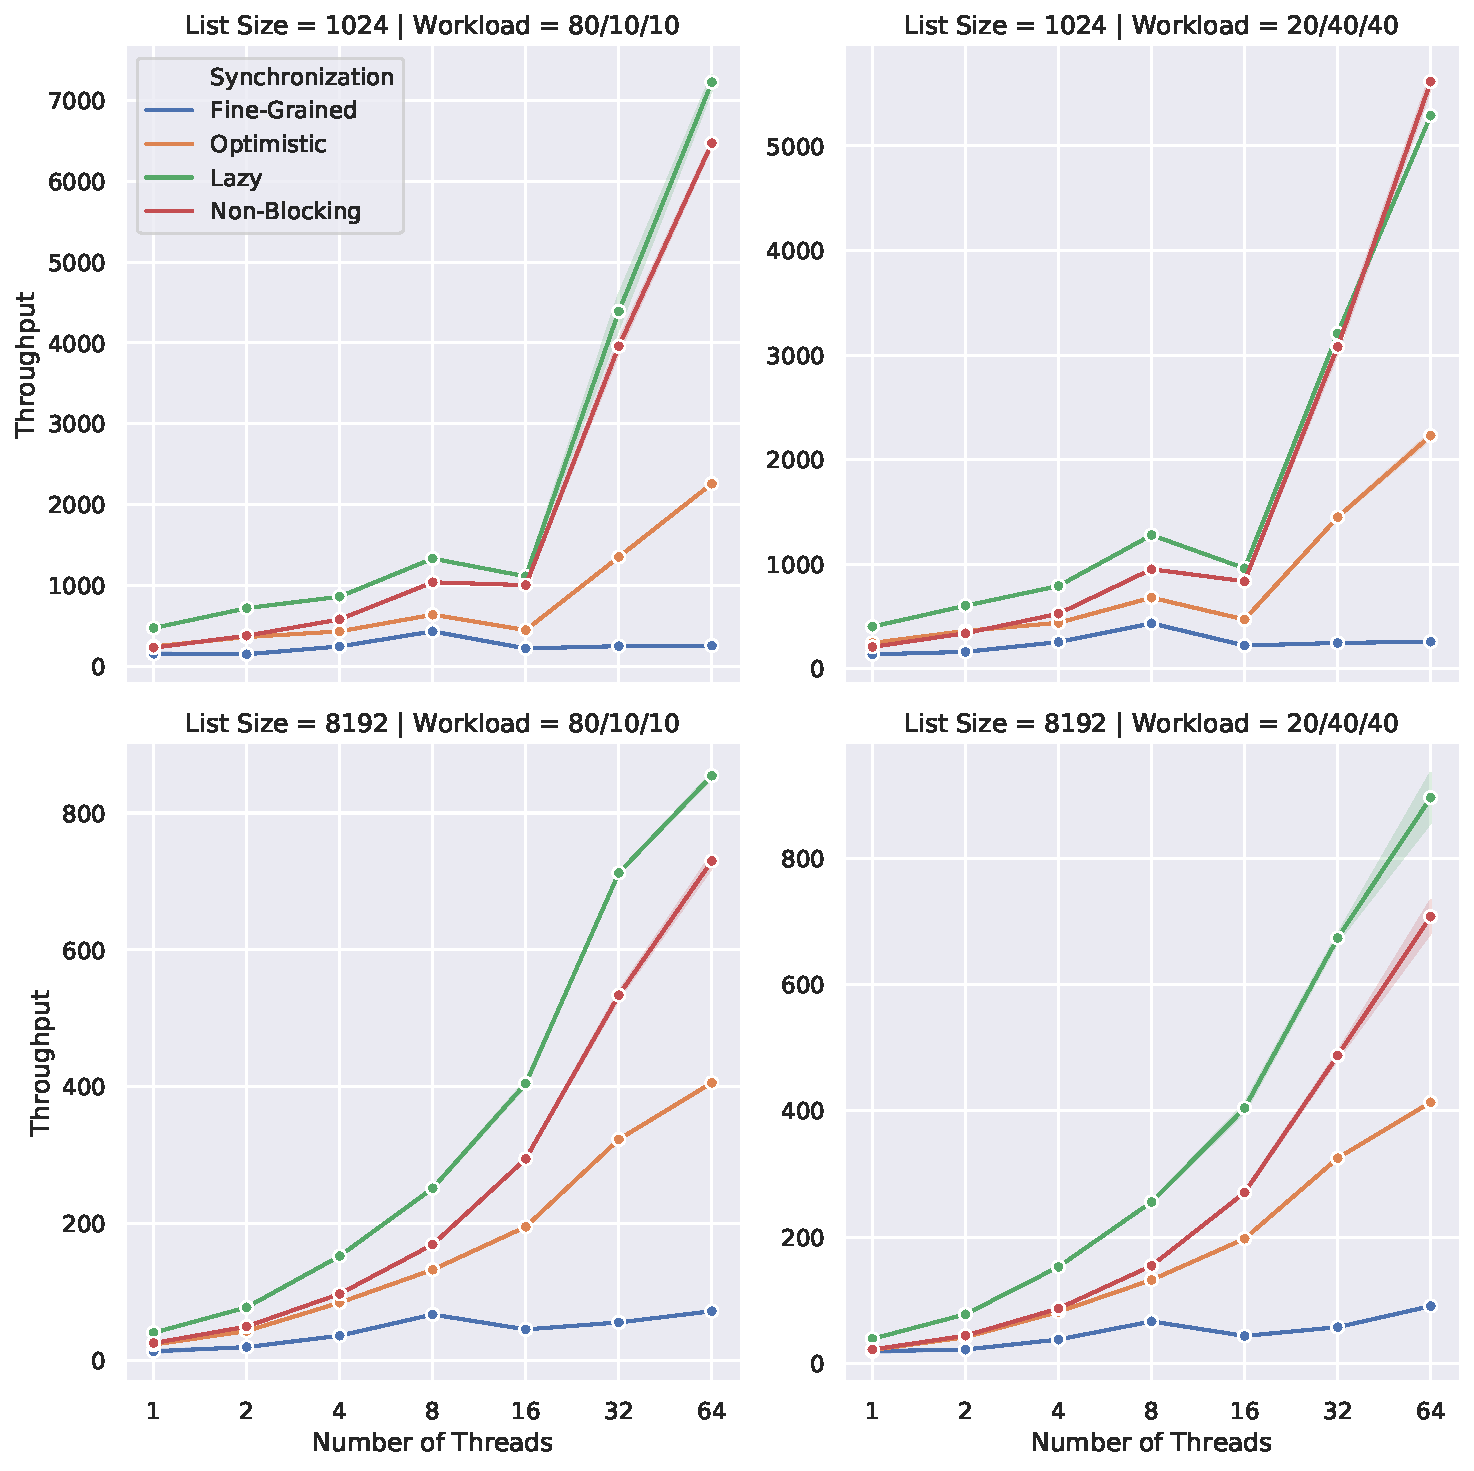
\includegraphics[width=\textwidth]{z3.pdf}
    \selectlanguage{greek}\caption{}
\end{figure}

Παρατηρούμε μια ξεκάθαρη διάταξη μεταξύ των τεχνικών που μελετήσαμε, η οποία σε
γενικές γραμμές είναι αυτή που αναμέναμε. Συγκεκριμένα η χειρότερη τακτική είναι
ο fine-grained συγχρονισμός, που υποφέρει από το overhead του hand-over-hand
locking. Ακολουθεί ο αισιόδοξος συγχρονισμός, που παρότι αισθητά καλύτερος,
σπαταλά πολύ χρόνο στη διάσχιση της λίστας από την αρχή για το validation. Οι 2
καλύτερες τακτικές είναι εμφανώς η οκνηρή και η non-blocking, με την πρώτη να
είναι αισθητά καλύτερη στην περίπτωση της μεγάλης λίστας.

Αξίζει να μελετήσουμε τη διαφορά μεταξύ των 2 καλύτερων υλοποιήσεων. Παρότι η
εξάλειψη των κλειδωμάτων είναι σημαντικό πλεονέκτημα, το τίμημα το οποίο
πληρώνουμε είναι η τροποποίηση της λίστας μέσω ατομικών (επομένως ακριβών)
εντολών σε μια packed δομή, η πρόσβαση στην οποία απαιτεί κάθε φορά unpacking.

Επιπλέον, το outsourcing της αφαίρεσης των σημειωμένων κόμβων στις add και
remove έχει ύπουλες παρενέργειες. Στην οκνηρή υλοποίηση οι συγκρούσεις
συνέβαιναν μεταξύ νημάτων που προσπαθούσαν να τροποποιήσουν τους ίδιους κόμβους,
πράγμα αρκετά σπάνιο. Επιπλέον σε μια πιο πολύπλοκη αλλά πιθανόν καλύτερη
υλοποίηση, οι πραγματικές αφαιρέσεις των κόμβων θα μπορούσαν να συμβαίνουν
μαζικά σε κατάλληλες στιμγές (λ.χ. όταν η δραστηριότητα των νημάτων αναφορικά με
τη λίστα είναι χαμηλή).

Αντίθετα, στο non-blocking συγχρονισμό τα νήματα πλέον είναι υποχρεωμένα να
σβήσουν κόμβους που δεν έχουν καμία σχέση με το στοιχείο που θέλουν να
τροποποιήσουν. Παύουν δηλαδή να είναι εντοπισμένα τα σημεία συγκρούσεων, με
αποτέλεσμα να αυξάνει η πιθανότητα σύγκρουσης και κατ' επέκταση η ανάγκη
επανεκκίνησης της διαδικασίας λόγω αποτυχίας.

Τα παραπάνω εξηγούν την υπεροχή της οκνηρής προσέγγισης. Εικάζουμε μάλιστα πως
στη μεγάλη λίστα η ακόμα μεγαλύτερη διαφορά οφείλεται στο αυξημένο (λόγω του
μεγέθους) κόστος των επανεκκινήσεων, που είναι σαφώς περισσότερες στην
non-blocking υλοποίηση.

Τέλος, αναφορικά με τα workloads, παρατηρούμε ότι δεν υπάρχει έντονη διαφορά.
Στο fine-grained και στον αισιόδοξο συγχρονισμό και οι 3 λειτουργίες
υλοποιούνται πανομοιότυπα (αναφορικά με τα κλειδώματα). Ως εκ τούτου, το
workload είναι αδιάφορο. Στην οκνηρή και τη non-blocking υλοποίηση από την άλλη
η contains είναι wait-free, ήτοι δεν περιέχει κανένα κλείδωμα (ή ατομική εντολή
ή retry). Ως εκ τούτου, αναμένουμε η ύπαρξη πολλών contains να αυξάνει το
throughput. Πράγματι διακρίνουμε μια τέτοια αισθητή διαφορά στην περίπτωση της
μικρής λίστας (ειδικά για 32 και 64 νήματα).

\end{document}